\documentclass[12pt]{article}
\usepackage[table]{xcolor}
\usepackage[shortlabels]{enumitem}
\usepackage{tabularx,xltabular}
\usepackage{graphicx}
\usepackage{hyperref}
\usepackage{verbatim}
\usepackage{geometry}
\usepackage{ulem}
\usepackage[official]{eurosym}
\usepackage{tikz}
\usetikzlibrary{arrows,backgrounds,calc,decorations.markings,patterns,3d}
\usepackage{pgfplots}
\pgfplotsset{compat = newest}
\usetikzlibrary{fit}
\newcommand\addvmargin[1]{
\usetikzlibrary{arrows}
\node[fit=(current bounding box),inner ysep=#1,inner xsep=0]{};}
\usepackage{cancel}
\usepackage{fontspec}
\usepackage{array}  
\geometry{a4paper, top=2cm, left=2cm, right=2cm, bottom=2cm, headsep=1cm}
\usepackage{tabu}
\usepackage{pst-node}
\usepackage{colortbl}
\usepackage{array}
\usepackage{german}
\setlength\parindent{0pt}
\newcolumntype{?}{!{\vrule width 1pt}}
\usepackage{makecell}
\renewcommand{\arraystretch}{2.5}
\usepackage{pbox}
\usepackage{amssymb}
\usepackage{amsmath}
\usepackage{booktabs}
\newcolumntype{L}[1]{>{\raggedright\let\newline\\\arraybackslash\hspace{0pt}}m{#1}}
\newcolumntype{C}[1]{>{\centering\let\newline\\\arraybackslash\hspace{0pt}}m{#1}}
\newcolumntype{R}[1]{>{\raggedleft\let\newline\\\arraybackslash\hspace{0pt}}m{#1}}
\begin{document}
\rightline{Datum: 08.06.2023}
\centerline{{\Large Tägliche Übungen}} 
\vspace{1cm}
\noindent \\


\begin{xltabular}{\textwidth}{|C{0.75cm}|X|C{0.75cm}|X|}
\arrayrulecolor{black}\hline
a)&$y:2=6$
&
b)&$y:9=5$
\\\hline
c)&$b:7=7$
&
d)&$y:4=7$
\\\hline
e)&$3\cdot b=33$
&
f)&$5\cdot a=10$
\\\hline
g)&$9\cdot a=27$
&
h)&$a:6=8$
\\\hline
i)&$3\cdot x=33$
&
j)&$x:5=10$
\\\hline
k)&$7\cdot x=49$
&
l)&$y:8=10$
\\\hline
m)&$b:2=2$
&
n)&$4\cdot x=32$
\\\hline
o)&$a:2=4$
&
p)&$a:11=6$
\\\hline
q)&$3\cdot x=36$
&
r)&$11\cdot a=22$
\\\hline
s)&$y:9=11$
&
t)&$y:6=3$
\\\hline
u)&$11\cdot a=55$
&
v)&$11\cdot a=88$
\\\hline
w)&$6\cdot a=30$
&
x)&$2\cdot x=14$
\\\hline
y)&$8\cdot y=56$
&
z)&$a:8=12$
\\\hline
\end{xltabular}
\vspace{0.5cm}
\newpage
\rightline{Datum: 08.06.2023}
\centerline{{\large Lösungen Tägliche Übungen}} 
\vspace{0.5cm}

\begin{xltabular}{\textwidth}{|C{0.75cm}|X|C{0.75cm}|X|}
\arrayrulecolor{black}\hline
a)&\begingroup\setlength{\jot}{-0.03cm}
\tikzstyle{background grid}=[draw, black!15,step=.5cm]
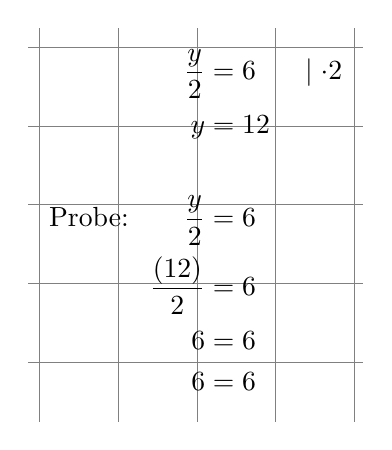
\begin{tikzpicture}[show background grid]
\node[below right] at (0,0.1) {
$\begin{aligned}
{{\frac{y}{2}}} &=6& & \mid \cdot 2\\
y &=12& & 
\\
\\
\mbox{Probe:}\qquad {{\frac{y}{2}}} &=6& &  \\
{{\frac{\left(12\right)}{2}}} &=6& &  \\
6 &=6& &  \\
6 &=6& &  \\
\end{aligned}$};
\end{tikzpicture}
\endgroup
&
b)&\begingroup\setlength{\jot}{-0.03cm}
\tikzstyle{background grid}=[draw, black!15,step=.5cm]
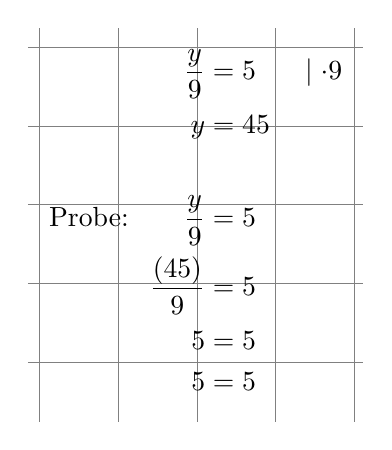
\begin{tikzpicture}[show background grid]
\node[below right] at (0,0.1) {
$\begin{aligned}
{{\frac{y}{9}}} &=5& & \mid \cdot 9\\
y &=45& & 
\\
\\
\mbox{Probe:}\qquad {{\frac{y}{9}}} &=5& &  \\
{{\frac{\left(45\right)}{9}}} &=5& &  \\
5 &=5& &  \\
5 &=5& &  \\
\end{aligned}$};
\end{tikzpicture}
\endgroup
\\\hline
c)&\begingroup\setlength{\jot}{-0.03cm}
\tikzstyle{background grid}=[draw, black!15,step=.5cm]
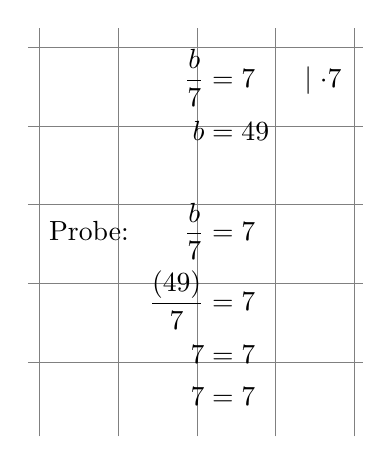
\begin{tikzpicture}[show background grid]
\node[below right] at (0,0.1) {
$\begin{aligned}
{{\frac{b}{7}}} &=7& & \mid \cdot 7\\
b &=49& & 
\\
\\
\mbox{Probe:}\qquad {{\frac{b}{7}}} &=7& &  \\
{{\frac{\left(49\right)}{7}}} &=7& &  \\
7 &=7& &  \\
7 &=7& &  \\
\end{aligned}$};
\end{tikzpicture}
\endgroup
&
d)&\begingroup\setlength{\jot}{-0.03cm}
\tikzstyle{background grid}=[draw, black!15,step=.5cm]
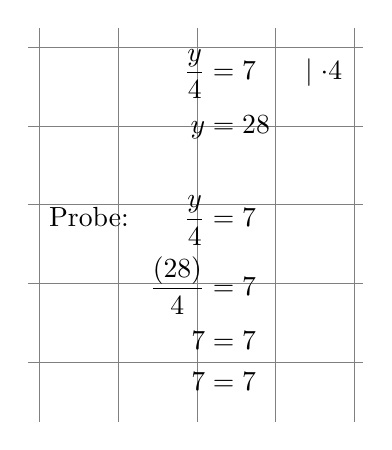
\begin{tikzpicture}[show background grid]
\node[below right] at (0,0.1) {
$\begin{aligned}
{{\frac{y}{4}}} &=7& & \mid \cdot 4\\
y &=28& & 
\\
\\
\mbox{Probe:}\qquad {{\frac{y}{4}}} &=7& &  \\
{{\frac{\left(28\right)}{4}}} &=7& &  \\
7 &=7& &  \\
7 &=7& &  \\
\end{aligned}$};
\end{tikzpicture}
\endgroup
\\\hline
e)&\begingroup\setlength{\jot}{-0.03cm}
\tikzstyle{background grid}=[draw, black!15,step=.5cm]
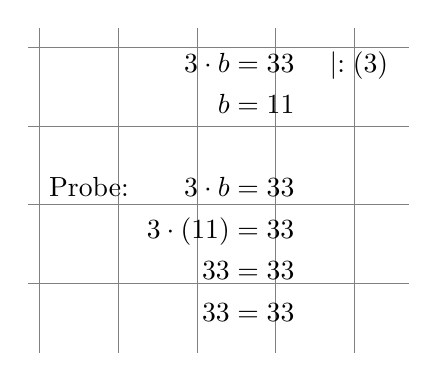
\begin{tikzpicture}[show background grid]
\node[below right] at (0,0.1) {
$\begin{aligned}
3\cdot b &=33& & \mid :\left(3\right)\\
b &=11& & 
\\
\\
\mbox{Probe:}\qquad 3\cdot b &=33& &  \\
3\cdot \left(11\right) &=33& &  \\
33 &=33& &  \\
33 &=33& &  \\
\end{aligned}$};
\end{tikzpicture}
\endgroup
&
f)&\begingroup\setlength{\jot}{-0.03cm}
\tikzstyle{background grid}=[draw, black!15,step=.5cm]
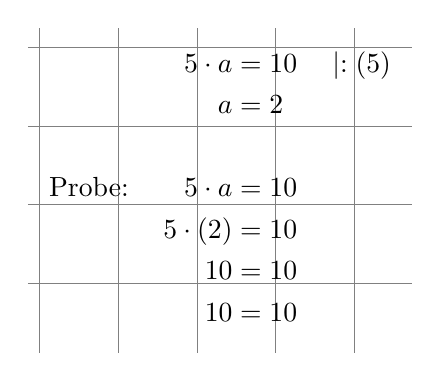
\begin{tikzpicture}[show background grid]
\node[below right] at (0,0.1) {
$\begin{aligned}
5\cdot a &=10& & \mid :\left(5\right)\\
a &=2& & 
\\
\\
\mbox{Probe:}\qquad 5\cdot a &=10& &  \\
5\cdot \left(2\right) &=10& &  \\
10 &=10& &  \\
10 &=10& &  \\
\end{aligned}$};
\end{tikzpicture}
\endgroup
\\\hline
g)&\begingroup\setlength{\jot}{-0.03cm}
\tikzstyle{background grid}=[draw, black!15,step=.5cm]
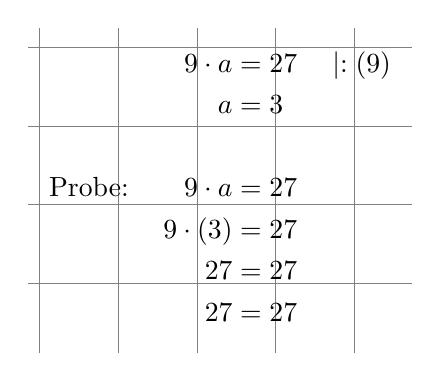
\begin{tikzpicture}[show background grid]
\node[below right] at (0,0.1) {
$\begin{aligned}
9\cdot a &=27& & \mid :\left(9\right)\\
a &=3& & 
\\
\\
\mbox{Probe:}\qquad 9\cdot a &=27& &  \\
9\cdot \left(3\right) &=27& &  \\
27 &=27& &  \\
27 &=27& &  \\
\end{aligned}$};
\end{tikzpicture}
\endgroup
&
h)&\begingroup\setlength{\jot}{-0.03cm}
\tikzstyle{background grid}=[draw, black!15,step=.5cm]
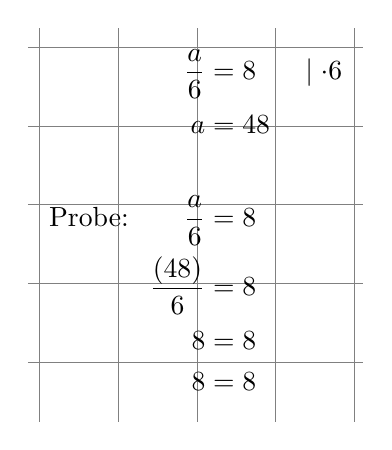
\begin{tikzpicture}[show background grid]
\node[below right] at (0,0.1) {
$\begin{aligned}
{{\frac{a}{6}}} &=8& & \mid \cdot 6\\
a &=48& & 
\\
\\
\mbox{Probe:}\qquad {{\frac{a}{6}}} &=8& &  \\
{{\frac{\left(48\right)}{6}}} &=8& &  \\
8 &=8& &  \\
8 &=8& &  \\
\end{aligned}$};
\end{tikzpicture}
\endgroup
\\\hline
i)&\begingroup\setlength{\jot}{-0.03cm}
\tikzstyle{background grid}=[draw, black!15,step=.5cm]
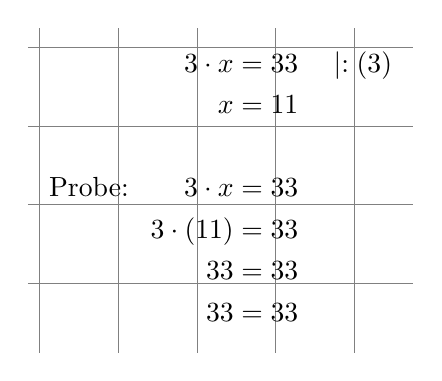
\begin{tikzpicture}[show background grid]
\node[below right] at (0,0.1) {
$\begin{aligned}
3\cdot x &=33& & \mid :\left(3\right)\\
x &=11& & 
\\
\\
\mbox{Probe:}\qquad 3\cdot x &=33& &  \\
3\cdot \left(11\right) &=33& &  \\
33 &=33& &  \\
33 &=33& &  \\
\end{aligned}$};
\end{tikzpicture}
\endgroup
&
j)&\begingroup\setlength{\jot}{-0.03cm}
\tikzstyle{background grid}=[draw, black!15,step=.5cm]
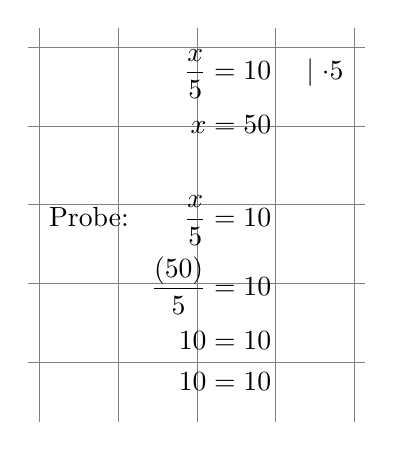
\begin{tikzpicture}[show background grid]
\node[below right] at (0,0.1) {
$\begin{aligned}
{{\frac{x}{5}}} &=10& & \mid \cdot 5\\
x &=50& & 
\\
\\
\mbox{Probe:}\qquad {{\frac{x}{5}}} &=10& &  \\
{{\frac{\left(50\right)}{5}}} &=10& &  \\
10 &=10& &  \\
10 &=10& &  \\
\end{aligned}$};
\end{tikzpicture}
\endgroup
\\\hline
k)&\begingroup\setlength{\jot}{-0.03cm}
\tikzstyle{background grid}=[draw, black!15,step=.5cm]
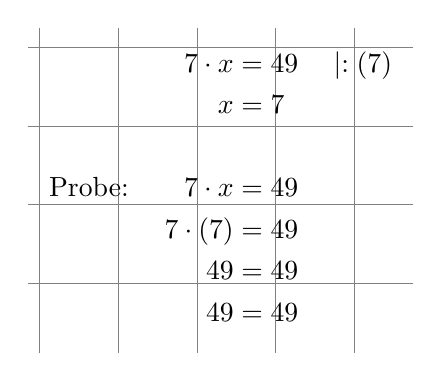
\begin{tikzpicture}[show background grid]
\node[below right] at (0,0.1) {
$\begin{aligned}
7\cdot x &=49& & \mid :\left(7\right)\\
x &=7& & 
\\
\\
\mbox{Probe:}\qquad 7\cdot x &=49& &  \\
7\cdot \left(7\right) &=49& &  \\
49 &=49& &  \\
49 &=49& &  \\
\end{aligned}$};
\end{tikzpicture}
\endgroup
&
l)&\begingroup\setlength{\jot}{-0.03cm}
\tikzstyle{background grid}=[draw, black!15,step=.5cm]
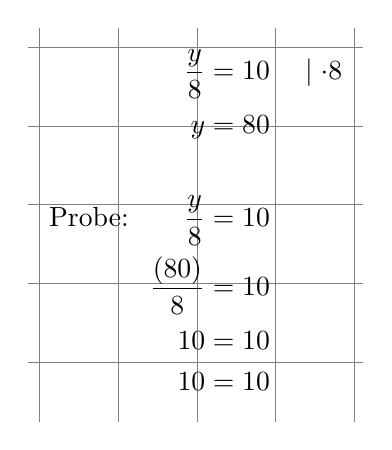
\begin{tikzpicture}[show background grid]
\node[below right] at (0,0.1) {
$\begin{aligned}
{{\frac{y}{8}}} &=10& & \mid \cdot 8\\
y &=80& & 
\\
\\
\mbox{Probe:}\qquad {{\frac{y}{8}}} &=10& &  \\
{{\frac{\left(80\right)}{8}}} &=10& &  \\
10 &=10& &  \\
10 &=10& &  \\
\end{aligned}$};
\end{tikzpicture}
\endgroup
\\\hline
m)&\begingroup\setlength{\jot}{-0.03cm}
\tikzstyle{background grid}=[draw, black!15,step=.5cm]
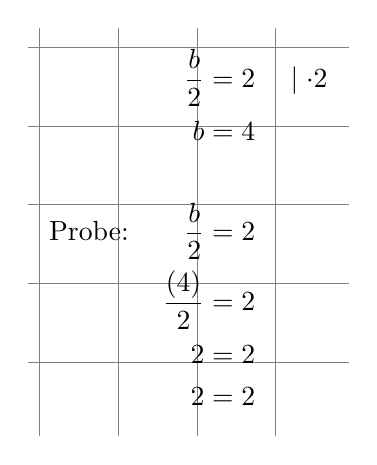
\begin{tikzpicture}[show background grid]
\node[below right] at (0,0.1) {
$\begin{aligned}
{{\frac{b}{2}}} &=2& & \mid \cdot 2\\
b &=4& & 
\\
\\
\mbox{Probe:}\qquad {{\frac{b}{2}}} &=2& &  \\
{{\frac{\left(4\right)}{2}}} &=2& &  \\
2 &=2& &  \\
2 &=2& &  \\
\end{aligned}$};
\end{tikzpicture}
\endgroup
&
n)&\begingroup\setlength{\jot}{-0.03cm}
\tikzstyle{background grid}=[draw, black!15,step=.5cm]
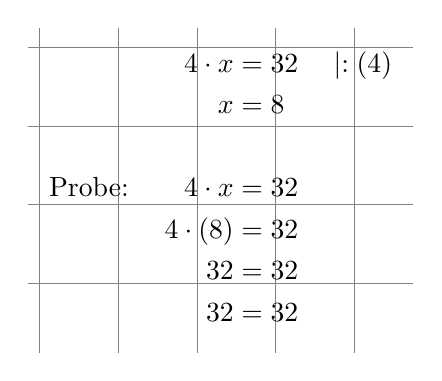
\begin{tikzpicture}[show background grid]
\node[below right] at (0,0.1) {
$\begin{aligned}
4\cdot x &=32& & \mid :\left(4\right)\\
x &=8& & 
\\
\\
\mbox{Probe:}\qquad 4\cdot x &=32& &  \\
4\cdot \left(8\right) &=32& &  \\
32 &=32& &  \\
32 &=32& &  \\
\end{aligned}$};
\end{tikzpicture}
\endgroup
\\\hline
o)&\begingroup\setlength{\jot}{-0.03cm}
\tikzstyle{background grid}=[draw, black!15,step=.5cm]
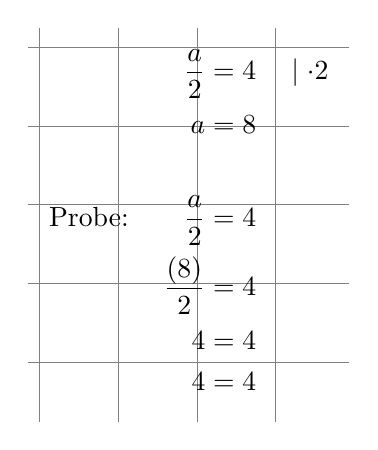
\begin{tikzpicture}[show background grid]
\node[below right] at (0,0.1) {
$\begin{aligned}
{{\frac{a}{2}}} &=4& & \mid \cdot 2\\
a &=8& & 
\\
\\
\mbox{Probe:}\qquad {{\frac{a}{2}}} &=4& &  \\
{{\frac{\left(8\right)}{2}}} &=4& &  \\
4 &=4& &  \\
4 &=4& &  \\
\end{aligned}$};
\end{tikzpicture}
\endgroup
&
p)&\begingroup\setlength{\jot}{-0.03cm}
\tikzstyle{background grid}=[draw, black!15,step=.5cm]
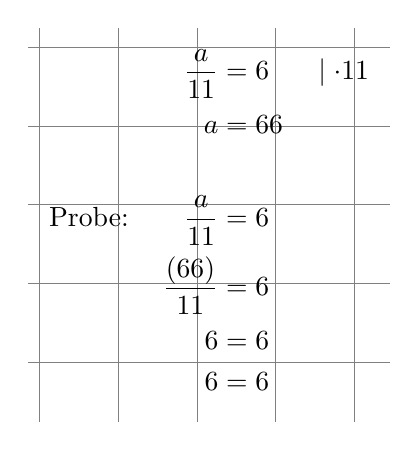
\begin{tikzpicture}[show background grid]
\node[below right] at (0,0.1) {
$\begin{aligned}
{{\frac{a}{11}}} &=6& & \mid \cdot 11\\
a &=66& & 
\\
\\
\mbox{Probe:}\qquad {{\frac{a}{11}}} &=6& &  \\
{{\frac{\left(66\right)}{11}}} &=6& &  \\
6 &=6& &  \\
6 &=6& &  \\
\end{aligned}$};
\end{tikzpicture}
\endgroup
\\\hline
q)&\begingroup\setlength{\jot}{-0.03cm}
\tikzstyle{background grid}=[draw, black!15,step=.5cm]
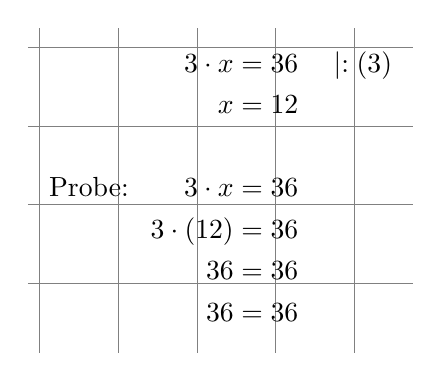
\begin{tikzpicture}[show background grid]
\node[below right] at (0,0.1) {
$\begin{aligned}
3\cdot x &=36& & \mid :\left(3\right)\\
x &=12& & 
\\
\\
\mbox{Probe:}\qquad 3\cdot x &=36& &  \\
3\cdot \left(12\right) &=36& &  \\
36 &=36& &  \\
36 &=36& &  \\
\end{aligned}$};
\end{tikzpicture}
\endgroup
&
r)&\begingroup\setlength{\jot}{-0.03cm}
\tikzstyle{background grid}=[draw, black!15,step=.5cm]
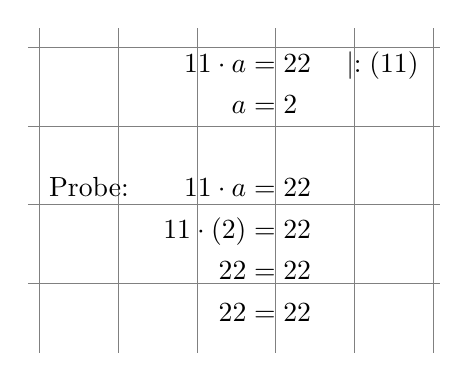
\begin{tikzpicture}[show background grid]
\node[below right] at (0,0.1) {
$\begin{aligned}
11\cdot a &=22& & \mid :\left(11\right)\\
a &=2& & 
\\
\\
\mbox{Probe:}\qquad 11\cdot a &=22& &  \\
11\cdot \left(2\right) &=22& &  \\
22 &=22& &  \\
22 &=22& &  \\
\end{aligned}$};
\end{tikzpicture}
\endgroup
\\\hline
s)&\begingroup\setlength{\jot}{-0.03cm}
\tikzstyle{background grid}=[draw, black!15,step=.5cm]
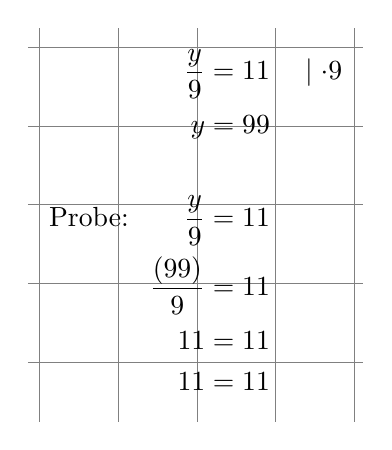
\begin{tikzpicture}[show background grid]
\node[below right] at (0,0.1) {
$\begin{aligned}
{{\frac{y}{9}}} &=11& & \mid \cdot 9\\
y &=99& & 
\\
\\
\mbox{Probe:}\qquad {{\frac{y}{9}}} &=11& &  \\
{{\frac{\left(99\right)}{9}}} &=11& &  \\
11 &=11& &  \\
11 &=11& &  \\
\end{aligned}$};
\end{tikzpicture}
\endgroup
&
t)&\begingroup\setlength{\jot}{-0.03cm}
\tikzstyle{background grid}=[draw, black!15,step=.5cm]
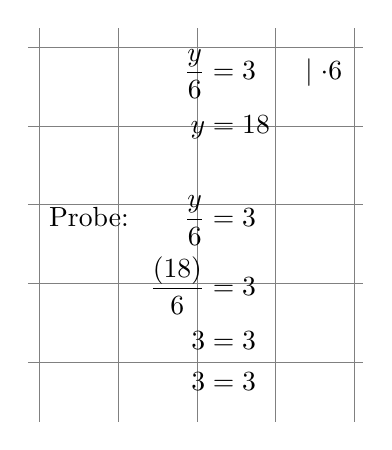
\begin{tikzpicture}[show background grid]
\node[below right] at (0,0.1) {
$\begin{aligned}
{{\frac{y}{6}}} &=3& & \mid \cdot 6\\
y &=18& & 
\\
\\
\mbox{Probe:}\qquad {{\frac{y}{6}}} &=3& &  \\
{{\frac{\left(18\right)}{6}}} &=3& &  \\
3 &=3& &  \\
3 &=3& &  \\
\end{aligned}$};
\end{tikzpicture}
\endgroup
\\\hline
u)&\begingroup\setlength{\jot}{-0.03cm}
\tikzstyle{background grid}=[draw, black!15,step=.5cm]
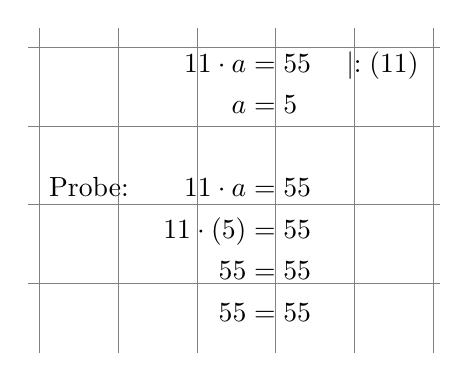
\begin{tikzpicture}[show background grid]
\node[below right] at (0,0.1) {
$\begin{aligned}
11\cdot a &=55& & \mid :\left(11\right)\\
a &=5& & 
\\
\\
\mbox{Probe:}\qquad 11\cdot a &=55& &  \\
11\cdot \left(5\right) &=55& &  \\
55 &=55& &  \\
55 &=55& &  \\
\end{aligned}$};
\end{tikzpicture}
\endgroup
&
v)&\begingroup\setlength{\jot}{-0.03cm}
\tikzstyle{background grid}=[draw, black!15,step=.5cm]
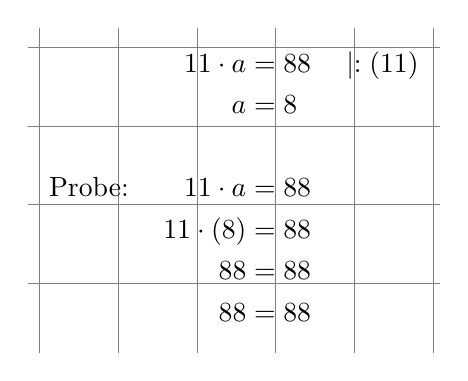
\begin{tikzpicture}[show background grid]
\node[below right] at (0,0.1) {
$\begin{aligned}
11\cdot a &=88& & \mid :\left(11\right)\\
a &=8& & 
\\
\\
\mbox{Probe:}\qquad 11\cdot a &=88& &  \\
11\cdot \left(8\right) &=88& &  \\
88 &=88& &  \\
88 &=88& &  \\
\end{aligned}$};
\end{tikzpicture}
\endgroup
\\\hline
w)&\begingroup\setlength{\jot}{-0.03cm}
\tikzstyle{background grid}=[draw, black!15,step=.5cm]
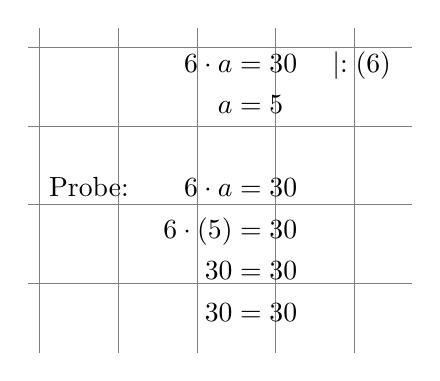
\begin{tikzpicture}[show background grid]
\node[below right] at (0,0.1) {
$\begin{aligned}
6\cdot a &=30& & \mid :\left(6\right)\\
a &=5& & 
\\
\\
\mbox{Probe:}\qquad 6\cdot a &=30& &  \\
6\cdot \left(5\right) &=30& &  \\
30 &=30& &  \\
30 &=30& &  \\
\end{aligned}$};
\end{tikzpicture}
\endgroup
&
x)&\begingroup\setlength{\jot}{-0.03cm}
\tikzstyle{background grid}=[draw, black!15,step=.5cm]
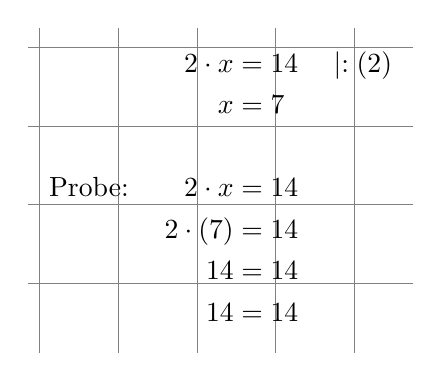
\begin{tikzpicture}[show background grid]
\node[below right] at (0,0.1) {
$\begin{aligned}
2\cdot x &=14& & \mid :\left(2\right)\\
x &=7& & 
\\
\\
\mbox{Probe:}\qquad 2\cdot x &=14& &  \\
2\cdot \left(7\right) &=14& &  \\
14 &=14& &  \\
14 &=14& &  \\
\end{aligned}$};
\end{tikzpicture}
\endgroup
\\\hline
y)&\begingroup\setlength{\jot}{-0.03cm}
\tikzstyle{background grid}=[draw, black!15,step=.5cm]
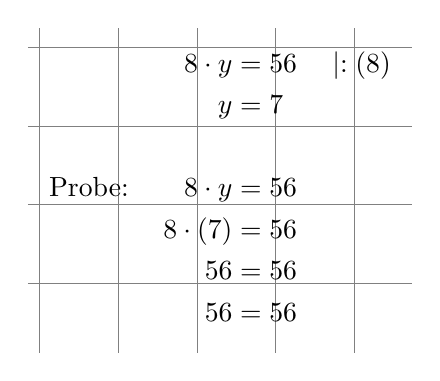
\begin{tikzpicture}[show background grid]
\node[below right] at (0,0.1) {
$\begin{aligned}
8\cdot y &=56& & \mid :\left(8\right)\\
y &=7& & 
\\
\\
\mbox{Probe:}\qquad 8\cdot y &=56& &  \\
8\cdot \left(7\right) &=56& &  \\
56 &=56& &  \\
56 &=56& &  \\
\end{aligned}$};
\end{tikzpicture}
\endgroup
&
z)&\begingroup\setlength{\jot}{-0.03cm}
\tikzstyle{background grid}=[draw, black!15,step=.5cm]
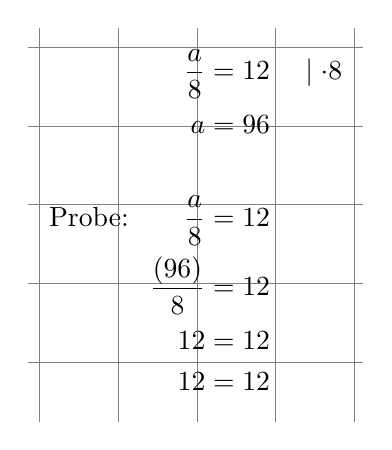
\begin{tikzpicture}[show background grid]
\node[below right] at (0,0.1) {
$\begin{aligned}
{{\frac{a}{8}}} &=12& & \mid \cdot 8\\
a &=96& & 
\\
\\
\mbox{Probe:}\qquad {{\frac{a}{8}}} &=12& &  \\
{{\frac{\left(96\right)}{8}}} &=12& &  \\
12 &=12& &  \\
12 &=12& &  \\
\end{aligned}$};
\end{tikzpicture}
\endgroup
\\\hline
\end{xltabular}
\vspace{0.5cm}
\end{document}